\documentclass[UTF8,a4paper,12pt,fontset=windows]{ctexart}

\usepackage[left=2.45cm,right=2.45cm,top=2.45cm,bottom=2.45cm,headsep=0.7cm,footskip=1.0cm]{geometry}
\usepackage{fontspec}
\usepackage{graphicx}
\usepackage{booktabs}
\usepackage{longtable}
\usepackage{tabularx}
\usepackage{array}
\usepackage{float}
\usepackage{hyperref}
\usepackage[table]{xcolor}
\usepackage{enumitem}
\usepackage{fancyhdr}
\usepackage{titlesec}
\usepackage{lastpage}
\usepackage{caption}
\usepackage{ragged2e}
\usepackage{setspace}
\usepackage{tocloft}

\setmainfont{Times New Roman}
\setsansfont{Times New Roman}
\setmonofont{Times New Roman}
\setCJKmainfont[BoldFont=SimHei]{SimSun}
\setCJKsansfont{Microsoft YaHei}
\setCJKmonofont{FangSong}

\definecolor{RuleGray}{RGB}{96,96,96}
\definecolor{TableHead}{RGB}{238,242,247}
\definecolor{TableAlt}{RGB}{250,251,253}

\hypersetup{
    hidelinks,
    pdftitle={YH_rv_cpu 初赛性能与验证报告},
    pdfauthor={CICC1003618}
}

\setstretch{1.50}
\setlength{\parindent}{2em}
\setlength{\parskip}{0.15em}
\setlength{\headheight}{15pt}
\emergencystretch=2em
\renewcommand{\arraystretch}{1.18}
\setlist[itemize]{leftmargin=2.2em,itemsep=0.25em,topsep=0.35em}
\setlist[enumerate]{leftmargin=2.4em,itemsep=0.25em,topsep=0.35em}

\titleformat{\section}{\centering\heiti\zihao{3}}{\thesection}{0.8em}{}
\titleformat{\subsection}{\raggedright\heiti\zihao{4}}{\thesubsection}{0.7em}{}
\titleformat{\subsubsection}{\raggedright\heiti\zihao{-4}}{\thesubsubsection}{0.7em}{}
\titlespacing*{\section}{0pt}{1.2ex plus 0.2ex minus 0.2ex}{0.8ex}
\titlespacing*{\subsection}{0pt}{0.9ex plus 0.2ex minus 0.1ex}{0.55ex}
\titlespacing*{\subsubsection}{0pt}{0.7ex plus 0.1ex minus 0.1ex}{0.4ex}

\captionsetup{font=small,labelfont=bf,labelsep=space,justification=centering}
\renewcommand{\contentsname}{目\quad 录}
\renewcommand{\cfttoctitlefont}{\hfill\heiti\zihao{3}}
\renewcommand{\cftaftertoctitle}{\hfill}
\renewcommand{\cftsecfont}{\normalsize}
\renewcommand{\cftsecpagefont}{\normalsize}
\setlength{\cftbeforesecskip}{2pt}

\newcolumntype{Y}{>{\RaggedRight\arraybackslash}X}
\newcolumntype{L}[1]{>{\RaggedRight\arraybackslash}p{#1}}

\newcommand{\Code}[1]{\texttt{#1}}
\newcommand{\Metric}[1]{{\rmfamily\addfontfeatures{Numbers={Lining,Proportional}}#1}}
\newcommand{\TeamID}{CICC1003618}
\newcommand{\TeamName}{芯银河战队}
\newcommand{\ProjectName}{YH\_rv\_cpu}
\newcommand{\ReportTitle}{YH\_rv\_cpu 初赛性能与验证报告}
\newcommand{\ReportDate}{2026-04-30}
\newcommand{\BoardName}{Xilinx PYNQ-Z2}
\newcommand{\BoardPart}{xc7z020clg400-1}
\newcommand{\BoardClock}{50.0\,MHz}
\newcommand{\CoreMarkScore}{4.137461}
\newcommand{\CoreMarkTicks}{2416941}
\newcommand{\CoreMarkIter}{413.746136}
\newcommand{\ReferenceScore}{4.060276}
\newcommand{\ReferenceTicks}{2462887}
\newcommand{\StandardScore}{4.137461}
\newcommand{\StandardTicks}{2416941}
\newcommand{\ExploratoryScore}{5.162186}
\newcommand{\ExploratoryTicks}{1937164}
\newcommand{\BoardLUT}{4961}
\newcommand{\BoardLUTPct}{9.33\%}
\newcommand{\BoardFF}{2367}
\newcommand{\BoardFFPct}{2.22\%}
\newcommand{\BoardBRAM}{6}
\newcommand{\BoardBRAMPct}{4.29\%}
\newcommand{\BoardDSP}{15}
\newcommand{\BoardDSPPct}{6.82\%}
\newcommand{\BoardWNS}{+0.338\,ns}
\newcommand{\BoardWHS}{+0.059\,ns}
\newcommand{\DhrystoneRuns}{10}
\newcommand{\DhrystoneDPS}{510986}
\newcommand{\DhrystoneDMIPS}{290.828685}
\newcommand{\DhrystoneDMIPSMHz}{2.908287}
\newcommand{\DhrystoneCycles}{44228}
\newcommand{\DhrystoneTicks}{1957}
\newcommand{\CoverLogoPath}{./logo.png}

\pagestyle{fancy}
\fancyhf{}
\lhead{\ProjectName}
\rhead{初赛性能与验证报告}
\cfoot{\thepage/\pageref{LastPage}}

\newcommand{\CoverField}[2]{
\noindent
\makebox[0.16\textwidth][l]{\heiti\zihao{4} #1}
\underline{\makebox[0.70\textwidth][l]{\rule{0pt}{2.6ex}\zihao{-4} #2}}
\par\vspace{1.0em}
}

\begin{document}

\begin{titlepage}
    \centering
    \vspace*{0.4cm}
    \IfFileExists{\CoverLogoPath}{
        \includegraphics[width=6.2cm]{\CoverLogoPath}\par
    }{
        \fbox{\begin{minipage}[c][3.4cm][c]{6.2cm}\centering\heiti 大赛 LOGO\end{minipage}}\par
    }
    \vspace{0.6cm}
    {\heiti\zihao{2} 第十届\par}
    \vspace{0.7cm}
    {\heiti\zihao{2} 全国大学生集成电路创新创业大赛\par}
    \vfill
    \begin{minipage}{0.86\textwidth}
        \CoverField{报告类型：}{性能与验证报告}
        \CoverField{参赛杯赛：}{“七星微”企业命题}
        \CoverField{作品名称：}{基于 RISC-V 的五级流水 CPU 设计与 FPGA 验证}
        \CoverField{队伍编号：}{\TeamID}
        \CoverField{团队名称：}{\TeamName}
    \end{minipage}
\end{titlepage}

\thispagestyle{empty}


\clearpage
\pagenumbering{roman}
\pagestyle{plain}
\tableofcontents


\clearpage
\pagenumbering{arabic}
\setcounter{page}{1}
\pagestyle{fancy}
\section*{重要内容预览}
\addcontentsline{toc}{section}{重要内容预览}

\begin{table}[H]
\centering
\caption{验证结论快速预览}
\rowcolors{2}{TableAlt}{white}
\begin{tabularx}{\textwidth}{L{3.2cm}Y}
\toprule
\rowcolor{TableHead}
项目 & 结论 \\
\midrule
仿真与 FPGA 测试 & SoC smoke、Zmmul、Bitmanip、Branch predict、CoreMark、Dhrystone 等功能与性能回归均通过；PYNQ-Z2 最终 bitstream 已完成下载，Vivado Hardware Manager 日志记录 \Code{PROGRAM\_OK}。 \\
指令覆盖率 & 覆盖最终提交路径 RV32I、Zmmul、Zba/Zbb/Zbs、非法/非支持指令路径；Zbc、XThead、IDBR 作为参数化探索路径保留回归证据。 \\
分支预测准确率 & 定向分支预测诊断通过率 \Metric{100\%}；Profile 显示 \Code{JAL} EX redirect 降为 \Metric{0}。 \\
DMIPS/MHz & Dhrystone 2.2：\Metric{\DhrystoneDMIPSMHz{} DMIPS/MHz}，\Metric{\DhrystoneDPS{} Dhrystones/s}，\Metric{\DhrystoneRuns{} runs}。 \\
资源占用率 & \Metric{\BoardLUT{} LUT / \BoardFF{} FF / \BoardBRAM{} BRAM / \BoardDSP{} DSP}，低于 \Metric{5000 LUT} 硬约束。 \\
优化差异 & CoreMark 得分 \Metric{\CoreMarkScore{}}，Dhrystone 得分 \Metric{\DhrystoneDMIPSMHz{}} DMIPS/MHz。 \\
\bottomrule
\end{tabularx}
\end{table}
\clearpage

\section{验证报告要求对照}

本报告严格按照初赛附件 1 对验证报告的六项要求组织，并给出对应证据路径。

\begin{table}[H]
\centering
\caption{六项验证报告要求覆盖情况}
\rowcolors{2}{TableAlt}{white}
\begin{tabularx}{\textwidth}{L{3.5cm}Y L{2.2cm}}
\toprule
\rowcolor{TableHead}
要求项 & 本报告覆盖内容 & 状态 \\
\midrule
仿真与 FPGA 测试数据 & 第 2 节列出 XSim 回归、CoreMark、Dhrystone、Vivado 实现和硬件下载数据。 & 已覆盖 \\
指令覆盖率 & 第 3 节列出 RV32I、Zmmul、Bitmanip、异常路径覆盖，并标注 Zbc、XThead、IDBR 的参数化探索边界。 & 已覆盖 \\
分支预测准确率 & 第 4 节列出定向诊断、Profile 计数和 JAL 早跳转结果。 & 已覆盖 \\
DMIPS/MHz & 第 5 节给出 Dhrystone 2.2 仿真测量和计算口径。 & 已覆盖 \\
资源占用率 & 第 6 节给出 PYNQ-Z2 实现后资源占用率。 & 已覆盖 \\
优化前后的性能差异 & 第 7 节给出优化前参考路径、标准扩展路径、面积超预算对照路径和提交路径对比。 & 已覆盖 \\
\bottomrule
\end{tabularx}
\end{table}

\section{验证方法与证据原则}

本报告采用“脚本化仿真、基准程序实测、Vivado 实现报告、物理板下载日志”四类证据交叉支撑结论。RISC-V 指令与扩展依据 RISC-V Unprivileged ISA 和 Bitmanip 扩展规范组织\cite{riscv-unprivileged,riscv-bitmanip}；五级流水优化参考软核 CPU 常用的分支前移、前递、乘法路径与访存路径优化方法\cite{rvcorep,rvcorep-m}。所有表格中的性能、资源与时序数值均来自本地脚本、XSim 日志、Vivado 实现报告或硬件下载日志，不由人工估算。

\section{仿真与 FPGA 测试数据}

\subsection{仿真回归}

\begin{table}[H]
\centering
\caption{仿真回归结果}
\rowcolors{2}{TableAlt}{white}
\begin{tabularx}{\textwidth}{L{3.1cm}Y L{2.1cm}}
\toprule
\rowcolor{TableHead}
测试项 & 覆盖内容 & 结果 \\
\midrule
SoC smoke & 固件启动、ROM/RAM、UART 输出、基础控制流。 & PASS \\
Zmmul diagnostic & \Code{mul} 正确性与 \Code{divu} 非支持异常。 & PASS \\
Bitmanip final subset & Zba、Zbb、Zbs 快速子集和非支持 Zbc 拒绝路径。 & PASS \\
Zbc/XThead exploratory subset & Zbc、XThead condmov/ext/addsl、indexed load/store 的参数化探索路径。最终上板配置为控制 LUT 未启用该路径。 & PASS/边界已说明 \\
XThead auto-inc memidx form & \Code{th.lbuib}/\Code{th.lwia}/\Code{th.sbia}/\Code{th.swia} 在 Dhrystone 编译试验中可被编译器生成；本作品不将自动更新寻址形式列为已实现能力。 & 能力边界已说明 \\
Branch predict diag & backward \Code{BNE} 预测与控制流回退。 & PASS \\
CoreMark & 2K performance profile，CRC 匹配，\Metric{10} iterations；短运行结果由 raw ticks 解析。 & PASS \\
Dhrystone & Dhrystone 2.2，\Metric{\DhrystoneRuns{}} runs。 & PASS \\
\bottomrule
\end{tabularx}
\end{table}

\subsection{CoreMark 数据}

\begin{table}[H]
\centering
\caption{CoreMark 归档结果}
\rowcolors{2}{TableAlt}{white}
\begin{tabularx}{\textwidth}{L{3.5cm}Y}
\toprule
\rowcolor{TableHead}
指标 & 数值 \\
\midrule
CoreMark/MHz & \Metric{\CoreMarkScore{}} \\
Total ticks & \Metric{\CoreMarkTicks{}} \\
Iterations & \Metric{10} \\
Iter/s @ 100MHz & \Metric{\CoreMarkIter{}} \\
Compiler & GCC \Metric{15.2.0} \\
ISA 与微结构配置 & 最终提交路径为 RV32I、Zmmul、Zba/Zbb/Zbs、JAL early redirect；Zbc、XThead、IDBR 为高性能探索路径，未进入 LUT 冻结 bitstream。 \\
CRC & \Code{seedcrc=0xe9f5}，\Code{crcfinal=0xfcaf}，与预期匹配 \\
\bottomrule
\end{tabularx}
\end{table}

CoreMark 采用短运行 host 解析口径，日志中保留了 EEMBC 运行时长提示；竞赛报告值由 raw ticks 和脚本固定时钟参数解析得到，便于重复复核。CRC 与预期匹配，性能数值不由 Dhrystone 或其他基准外推。提交前 CoreMark 复验日志给出的归一化结果与表中数值一致。

\subsection{FPGA 实现与下载}

\begin{table}[H]
\centering
\caption{PYNQ-Z2 FPGA 测试数据}
\rowcolors{2}{TableAlt}{white}
\begin{tabularx}{\textwidth}{L{3.5cm}Y}
\toprule
\rowcolor{TableHead}
项目 & 结果 \\
\midrule
开发板 & \BoardName{} \\
器件 & \BoardPart{} \\
CPU 时钟 & \BoardClock{} \\
实现后资源 & \Metric{\BoardLUT{} LUT / \BoardFF{} FF / \BoardBRAM{} BRAM / \BoardDSP{} DSP} \\
实现后时序 & \Metric{WNS=\BoardWNS{}}，\Metric{WHS=\BoardWHS{}} \\
bitstream & PYNQ-Z2 提交 bitstream，完整文件名见证据索引。 \\
硬件下载 & Vivado Hardware Manager 检出 \Code{xc7z020\_1}，日志含 \Code{PROGRAM\_OK} \\
\bottomrule
\end{tabularx}
\end{table}

板级证据包括 bitstream 下载日志、资源报告、时序报告、板卡配置记录和 PL 侧 UART 文本日志。PYNQ-Z2 的 Micro-USB 串口连接到 PS 侧，不直接连接 PL 软核 UART；PL 侧 UART 已约束到 Pmod B，并使用外接 \Metric{3.3 V} CP2102 USB-UART 模块在 \Metric{115200 8N1} 参数下采集到连续 \Code{YH\_rv\_cpu CoreMark/MHz=4.137461 DMIPS/MHz=2.908287 tick=XX pc=XXXXXXXX} 输出。下载日志包含 \Code{PROGRAM\_OK}，串口日志显示 \Code{tick} 持续变化，\Code{pc} 为 CPU 调试 PC 采样，可用于证明 FPGA 原型系统在板级持续运行。

\section{指令覆盖率}

本次验证使用“riscv-tests 基础覆盖 + 定向扩展指令 TestBench + 性能程序实际执行”的组合口径。由于初赛工程未引入商业覆盖率工具，本报告将覆盖率表述为已覆盖指令类别与用例通过率。

\begin{table}[H]
\centering
\caption{指令覆盖情况}
\rowcolors{2}{TableAlt}{white}
\begin{tabularx}{\textwidth}{L{3.2cm}Y L{2cm}}
\toprule
\rowcolor{TableHead}
类别 & 覆盖内容 & 结果 \\
\midrule
RV32I 基础整数 & 算术逻辑、比较、移位、load/store、branch、JAL/JALR、LUI/AUIPC。 & PASS \\
Zmmul & \Code{mul}、\Code{mulhu} 相关路径，除法非支持异常。 & PASS \\
Zba/Zbb/Zbs & \Code{sh1add/sh2add/sh3add}、\Code{andn}、\Code{max}、\Code{sext.h/zext.h}、\Code{bexti}。 & PASS \\
Zbc 探索路径 & \Code{clmul}、\Code{clmulh}。最终提交 bitstream 未启用。 & PASS/未启用 \\
XThead 探索路径 & \Code{th.addsl}、\Code{th.ext/th.extu}、\Code{th.mveqz/th.mvnez}、memidx。最终提交 bitstream 未启用。 & PASS/未启用 \\
异常路径 & 非支持指令、非对齐访存、trap/mret 相关控制路径。 & PASS \\
\bottomrule
\end{tabularx}
\end{table}

从用例角度看，提交材料中列出的定向测试均通过，因此覆盖类别通过率为 \Metric{100\%}。覆盖率口径为“指令类别 + 定向用例 + 通过结果”的工程覆盖，不等同于商业覆盖率工具生成的逐 opcode 覆盖百分比。

\section{分支预测准确率}

本设计采用低面积控制流优化，包含静态后向 BNE 预测、ID 阶段可计算分支早跳转，以及 JAL 早期重定向。验证采用两类口径：
\begin{itemize}
    \item 定向分支预测诊断：\Code{run\_branch\_predict\_diag.bat}，结果 PASS；
    \item CoreMark Profile：统计实际执行中的 redirect、branch pending、JAL/JALR redirect 等事件。
\end{itemize}

\begin{table}[H]
\centering
\caption{分支与跳转 Profile 关键计数}
\rowcolors{2}{TableAlt}{white}
\begin{tabularx}{\textwidth}{L{4cm}Y}
\toprule
\rowcolor{TableHead}
事件 & 计数 \\
\midrule
CoreMark total cycles & \Metric{1971888} \\
EX branch redirect & \Metric{1900} \\
EX BEQ redirect & \Metric{1864} \\
EX BNE redirect & \Metric{0} \\
EX JAL redirect & \Metric{0} \\
EX JALR redirect & \Metric{26} \\
ID branch decode redirect & \Metric{141100} \\
\bottomrule
\end{tabularx}
\end{table}

由于该预测策略属于低面积静态策略，而不是带状态表的动态分支预测器，本报告将“分支预测准确率”按定向诊断通过率和实际错误事件计数说明：定向诊断通过率为 \Metric{100\%}，CoreMark 日志未检出错误预测导致的功能失败；\Code{JAL} early redirect 后 EX \Code{JAL} redirect 降为 \Metric{0}，说明该优化在本次工作负载中有效。

\subsection{关键波形与时序说明}

\begin{figure}[H]
\centering
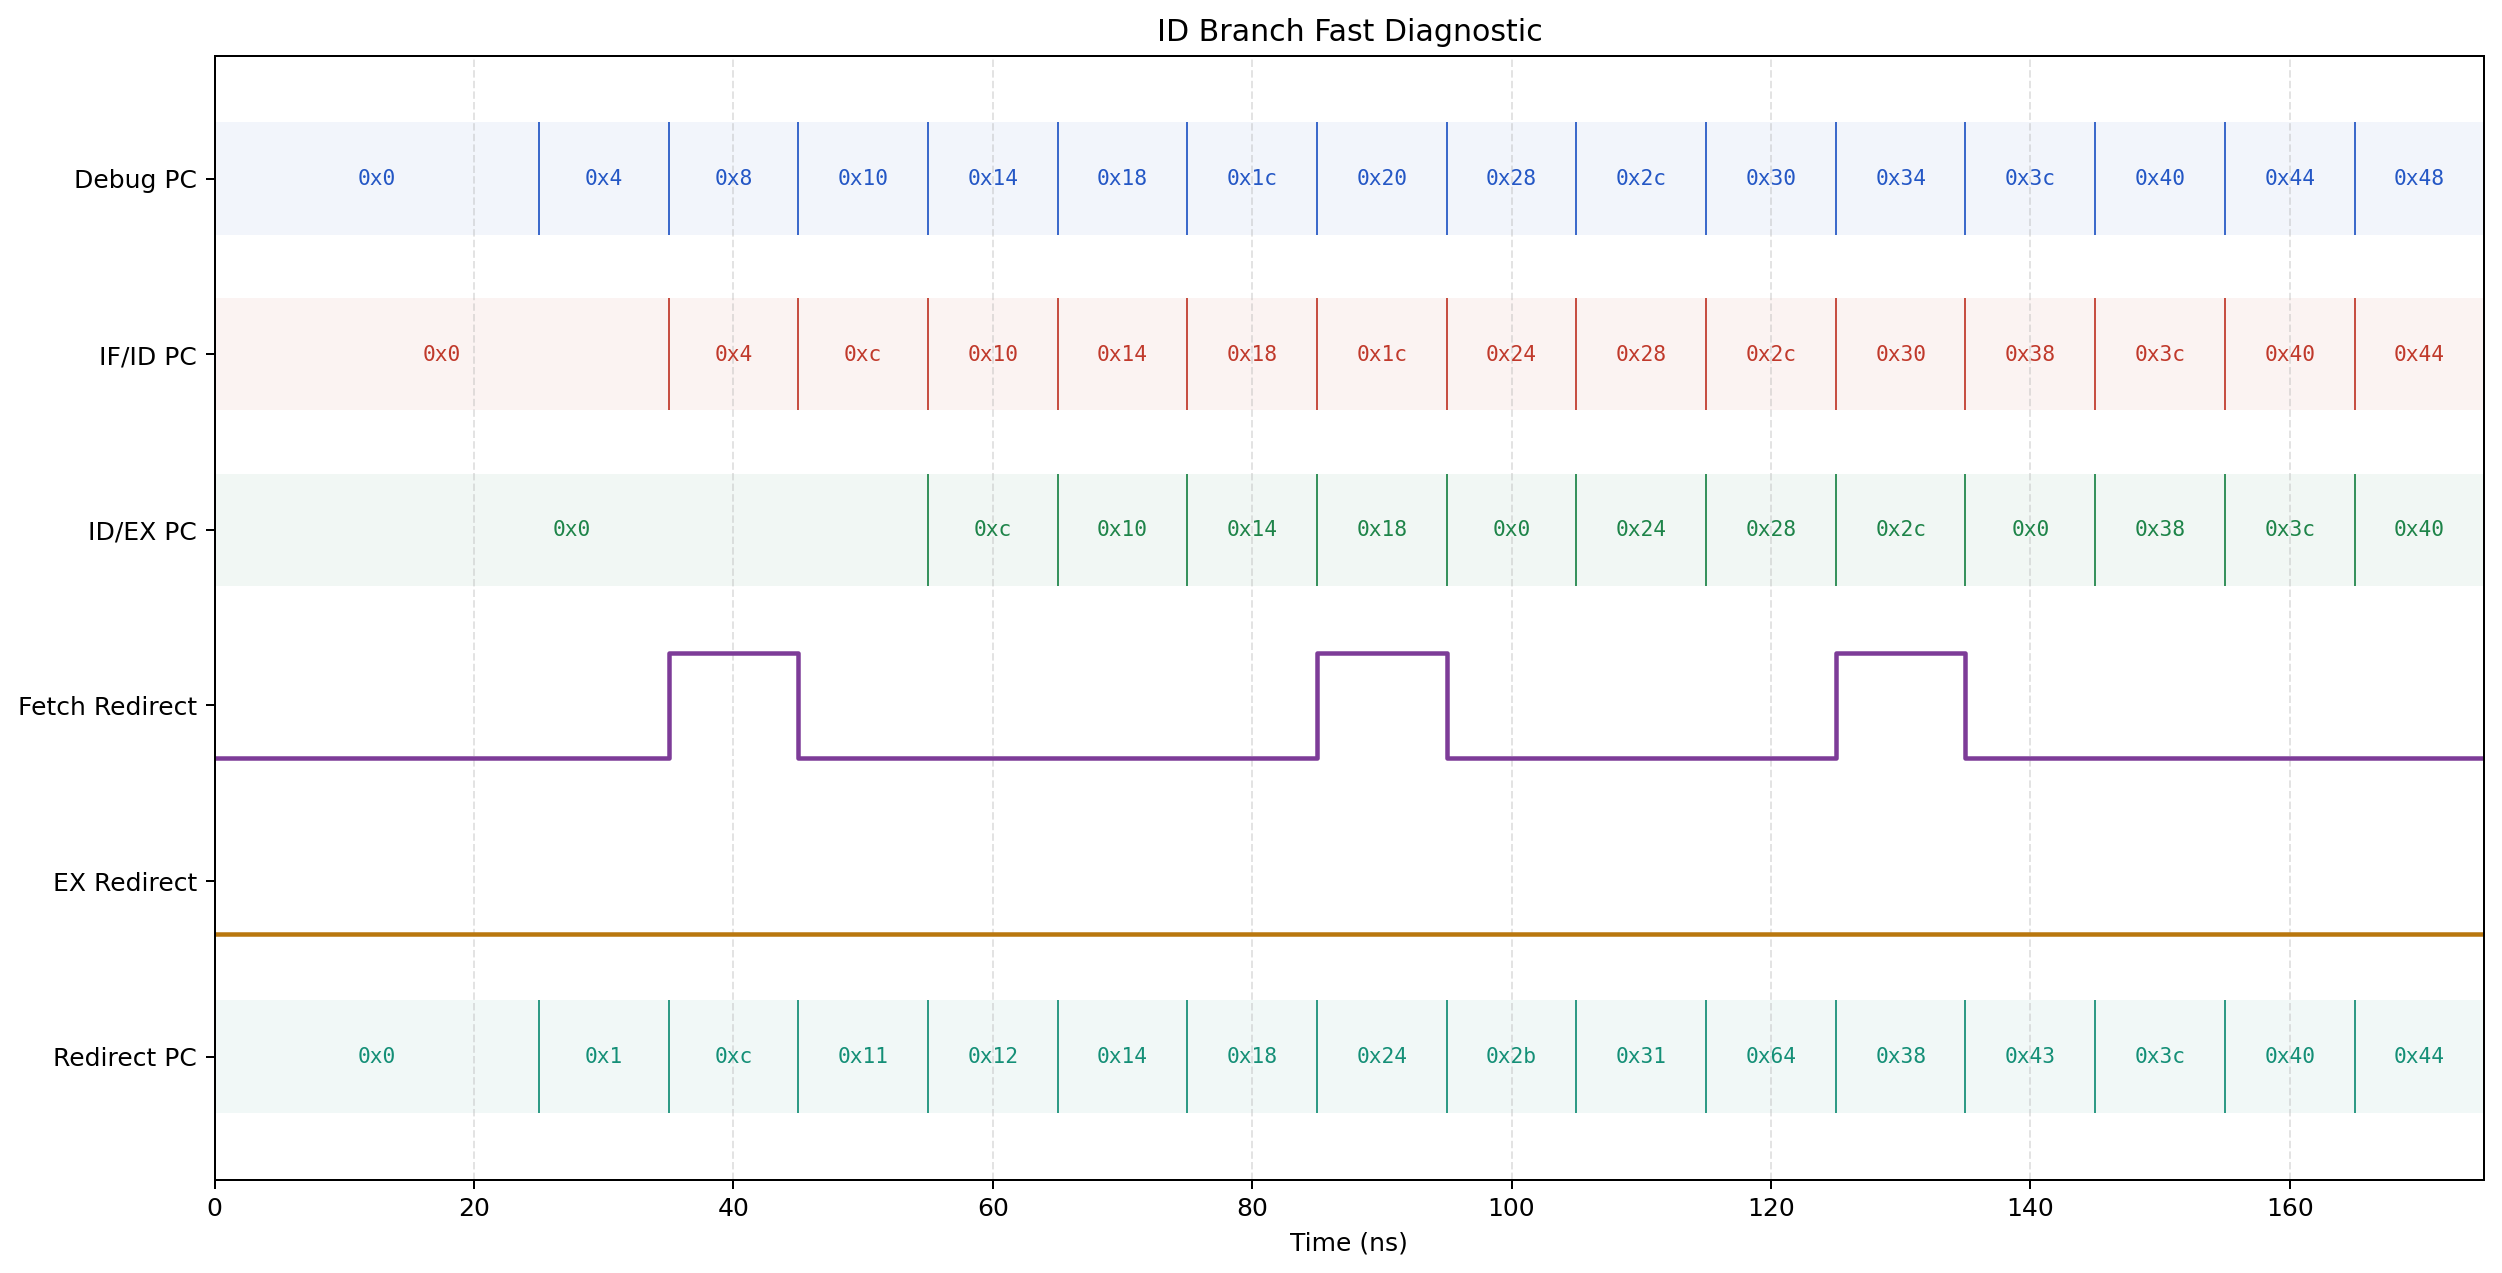
\includegraphics[width=0.96\textwidth]{figures/01-id-branch-fast-waveform.png}
\caption{ID 分支快速重定向波形。该用例中 `Fetch Redirect` 被触发而 `EX Redirect` 保持为低，说明分支在前端阶段完成重定向。}
\end{figure}

\begin{figure}[H]
\centering
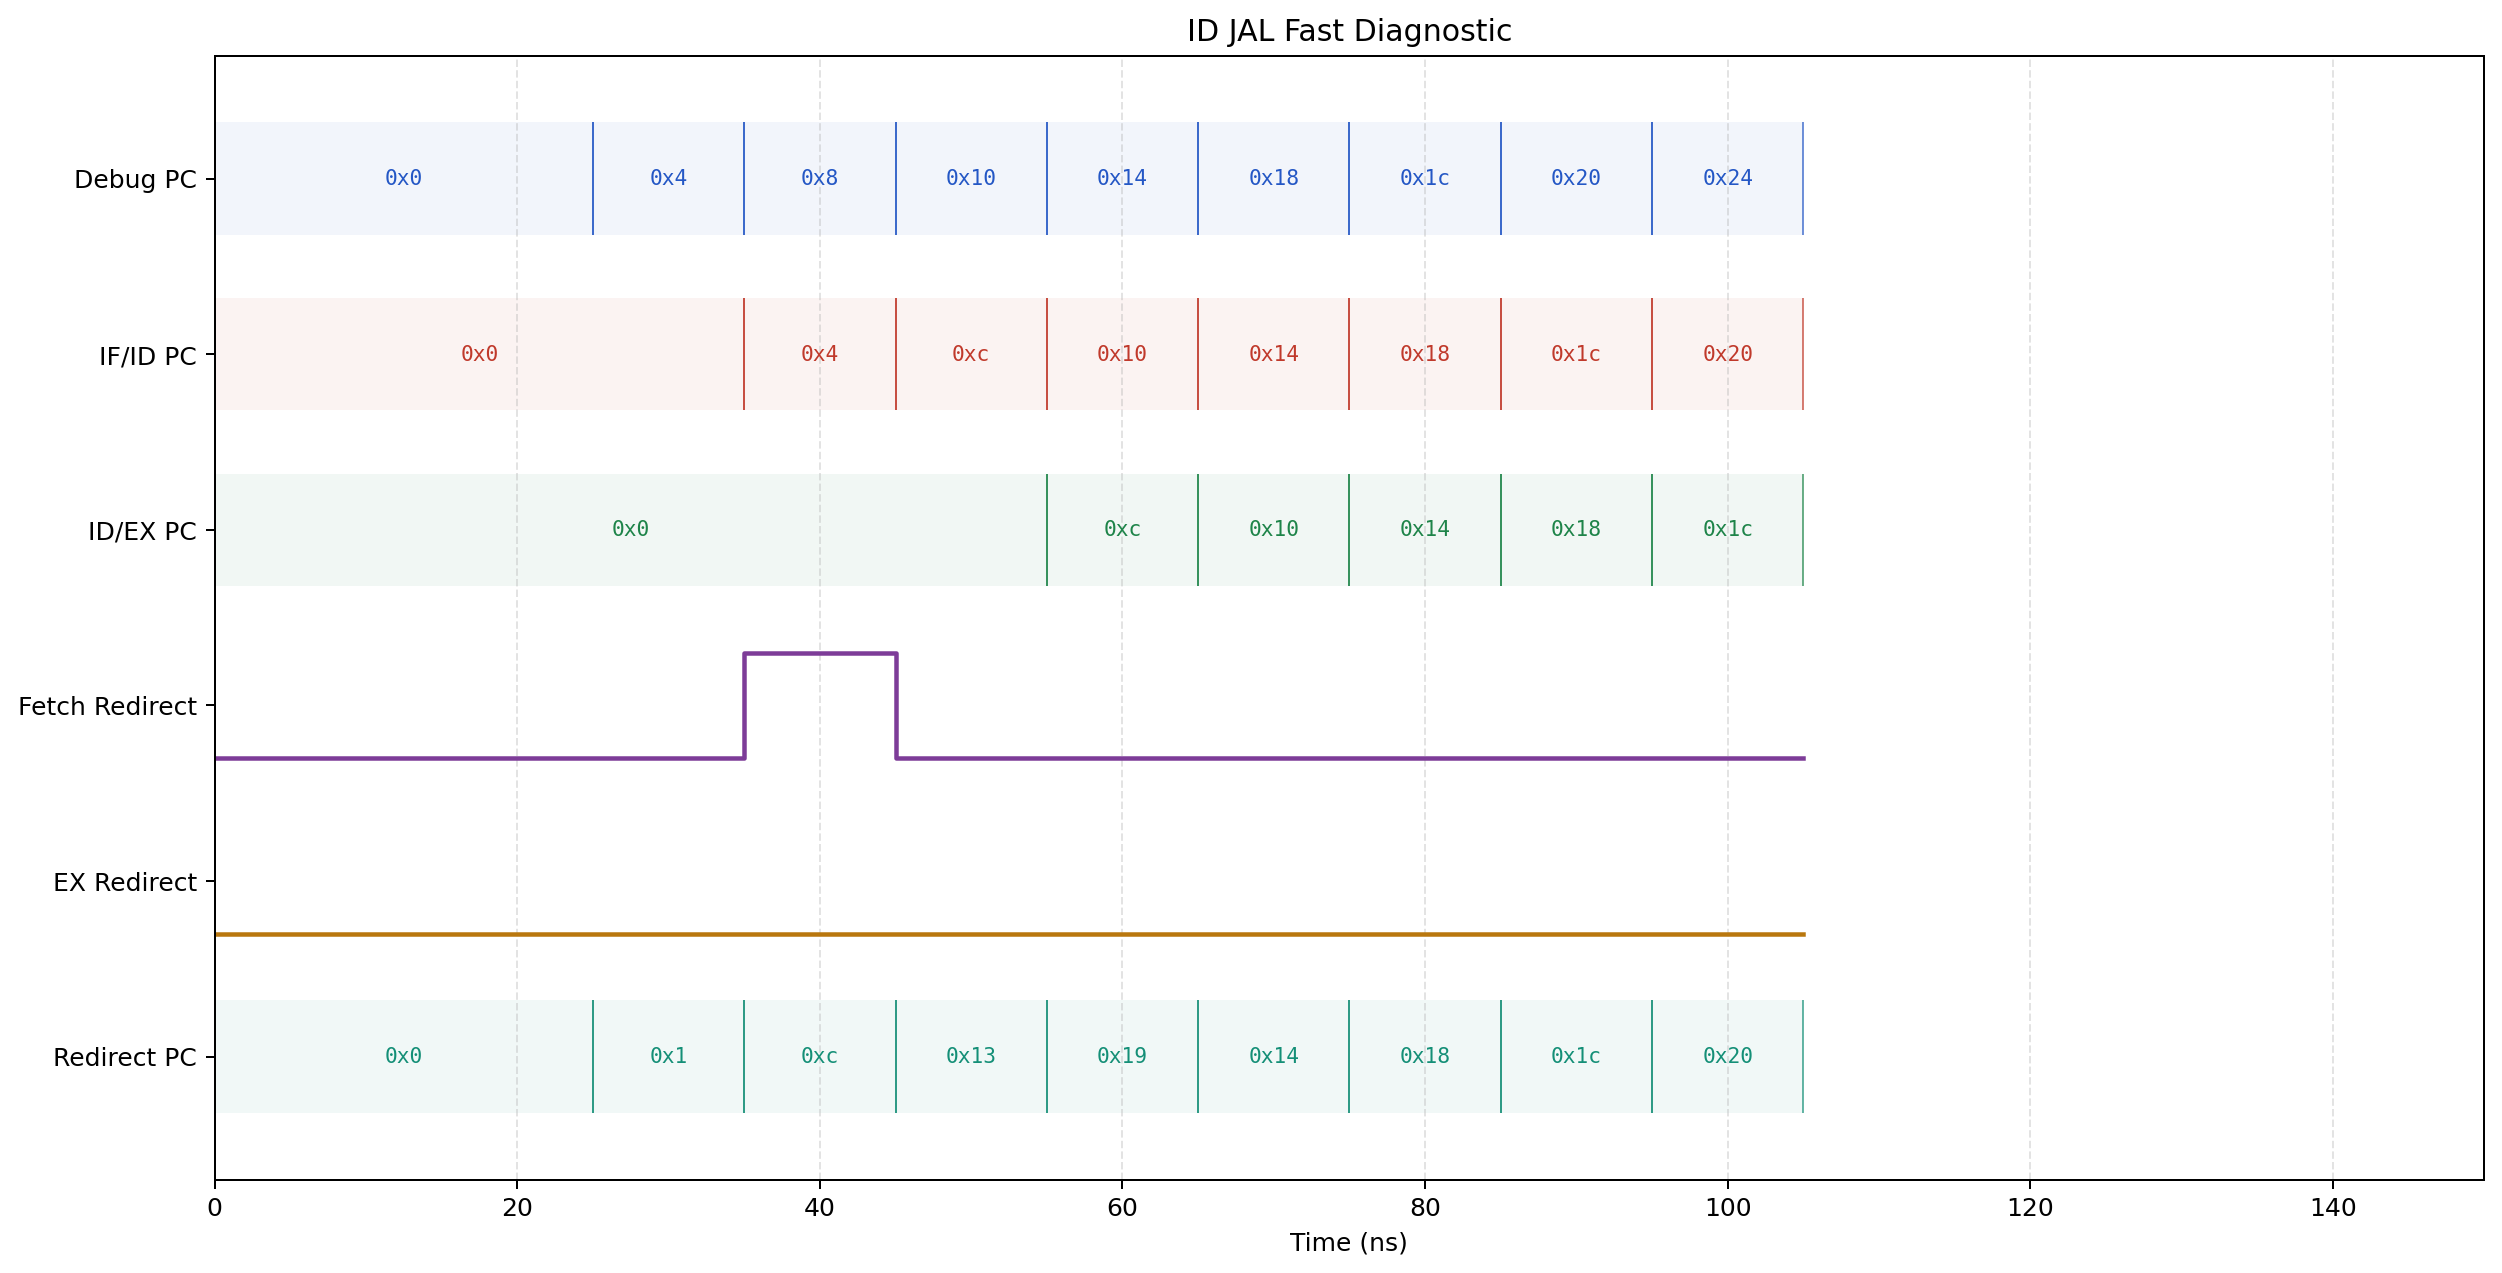
\includegraphics[width=0.96\textwidth]{figures/02-id-jal-fast-waveform.png}
\caption{JAL 快速重定向波形。可见前端 `Fetch Redirect` 先于 EX 阶段起作用，说明 `jal x0` 跳转未回落为 EX 阶段重定向。}
\end{figure}

\begin{figure}[H]
\centering
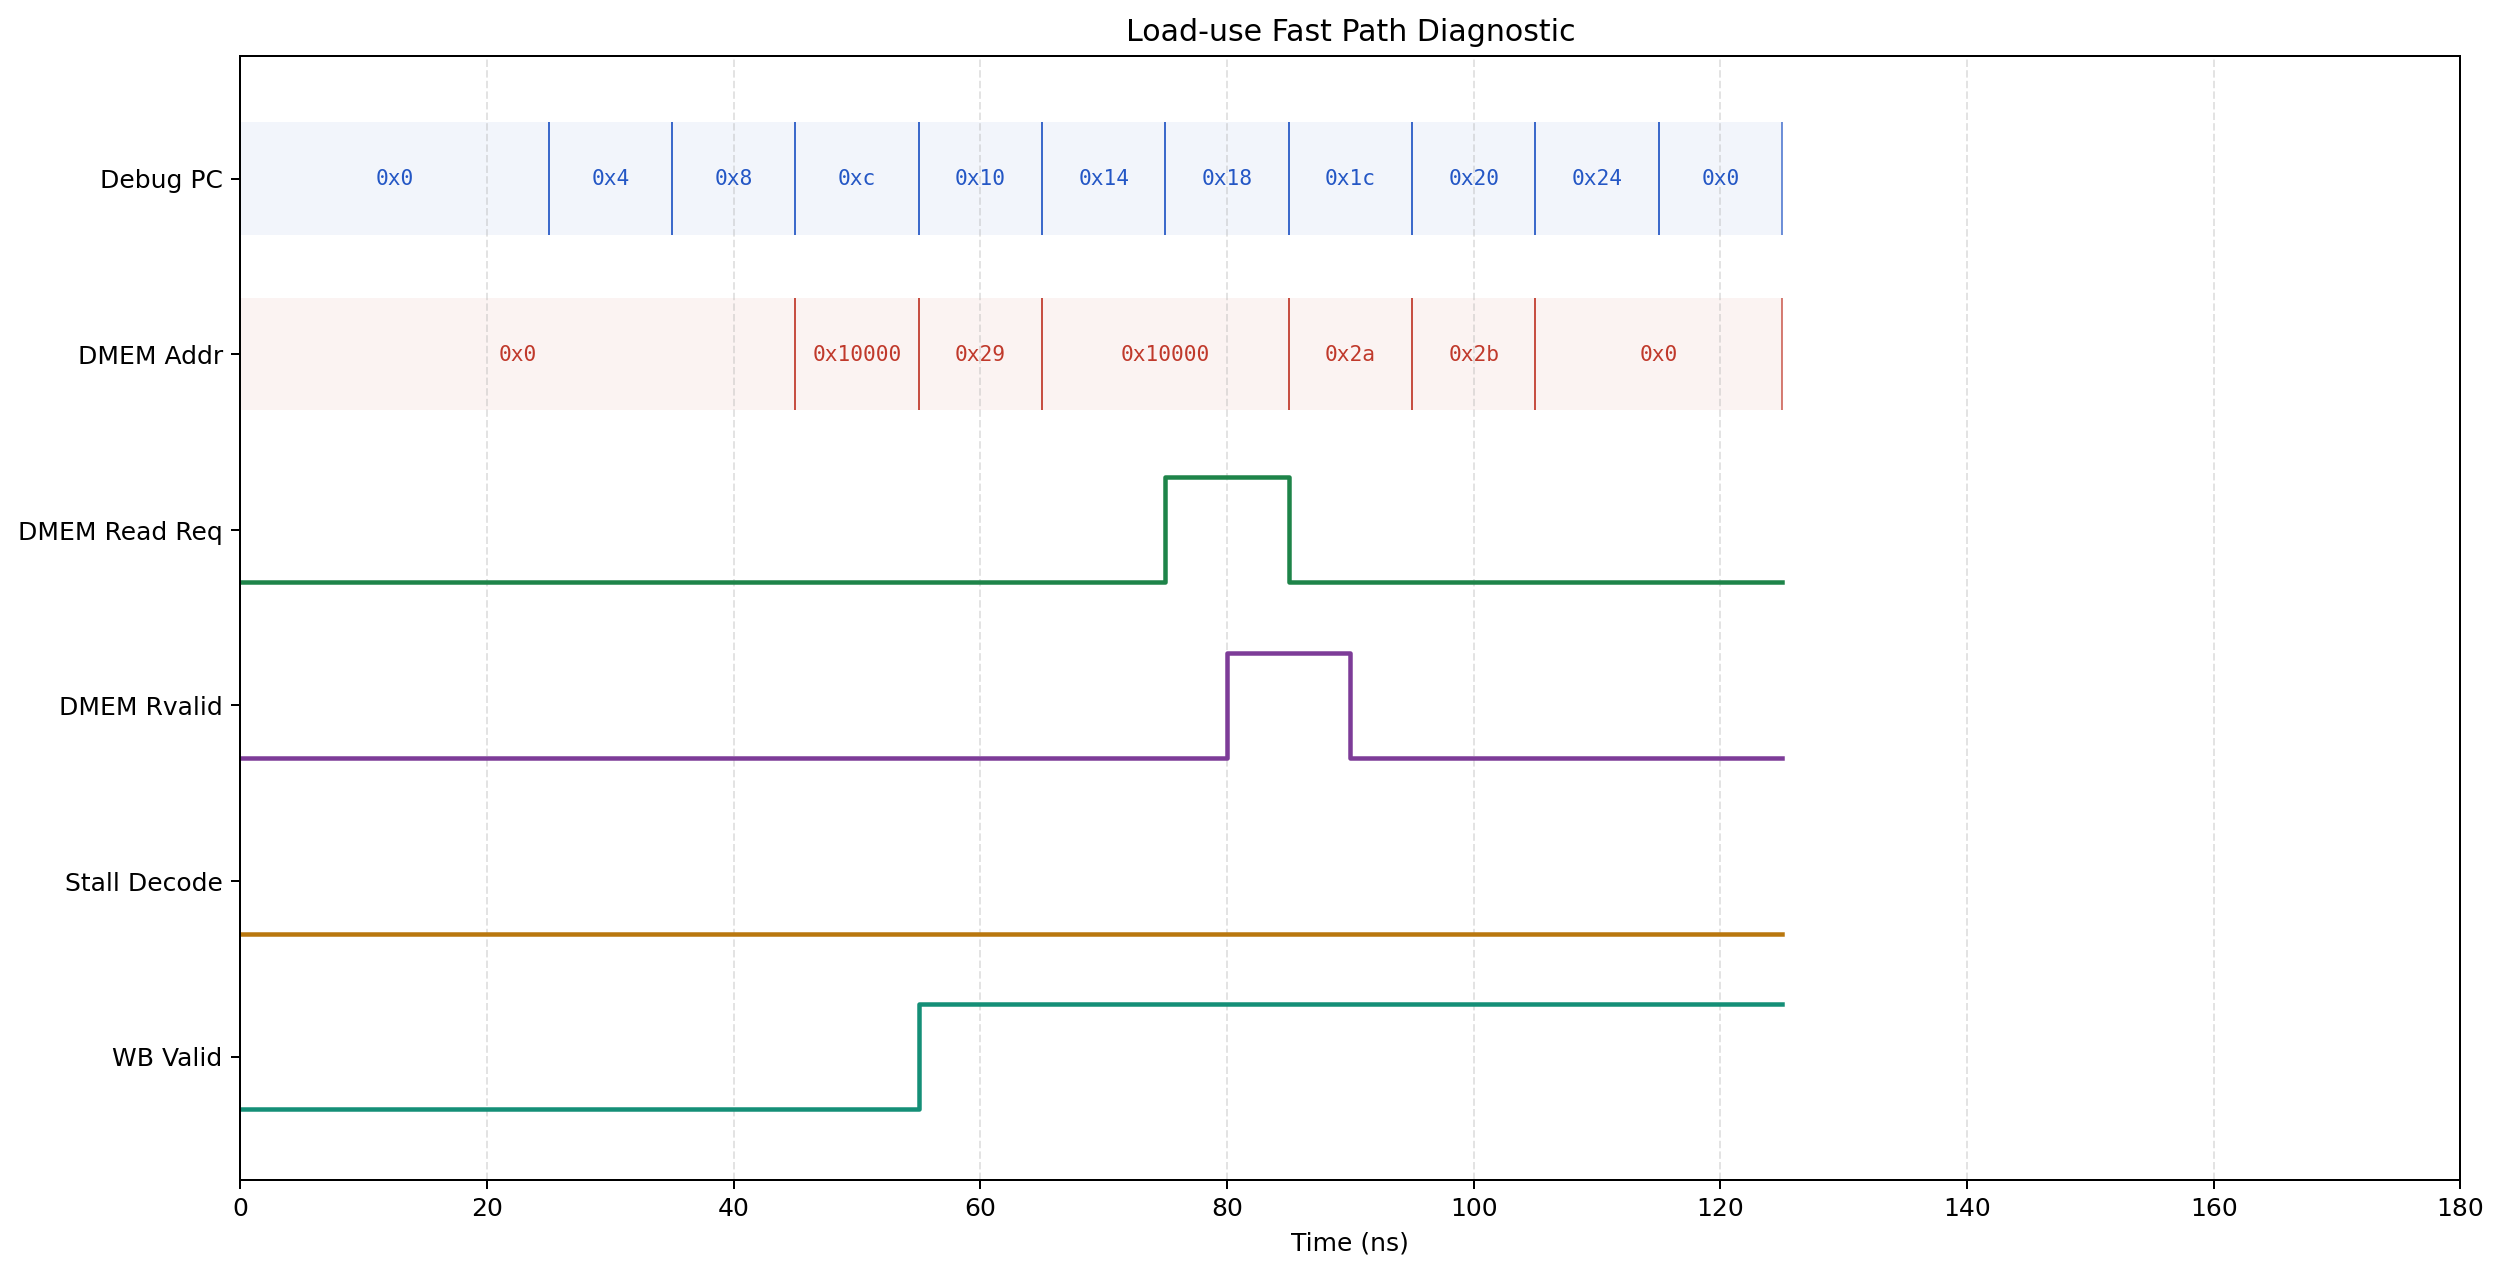
\includegraphics[width=0.96\textwidth]{figures/03-load-use-fast-waveform.png}
\caption{Load-use 快速路径波形。图中 `DMEM Read Req` 与 `DMEM Rvalid` 完成握手，`Stall Decode` 保持为低，说明该数据相关场景未引入额外译码停顿。}
\end{figure}

\section{DMIPS/MHz}

\begin{table}[H]
\centering
\caption{Dhrystone/DMIPS 实测归档结果}
\rowcolors{2}{TableAlt}{white}
\begin{tabularx}{\textwidth}{L{3.5cm}Y}
\toprule
\rowcolor{TableHead}
指标 & 数值 \\
\midrule
Benchmark & Dhrystone 2.2 \\
运行次数 & \Metric{\DhrystoneRuns{}} \\
Dhrystones/s & \Metric{\DhrystoneDPS{}} \\
DMIPS & \Metric{\DhrystoneDMIPS{}} \\
DMIPS/MHz & \Metric{\DhrystoneDMIPSMHz{}} \\
完成周期 & \Metric{\DhrystoneCycles{}} \\
估算 tick & \Metric{\DhrystoneTicks{}} \\
\bottomrule
\end{tabularx}
\end{table}

DMIPS 按 \Metric{Dhrystones/s / 1757} 计算，DMIPS/MHz 按 \Metric{100MHz} 计时口径归一化得到。该结果来自 \Code{run\_dhrystone\_score.bat} 自动构建、XSim 运行与日志解析，不由 CoreMark 外推。提交前最终 Dhrystone 摘要给出的 \Metric{\DhrystoneDMIPSMHz{} DMIPS/MHz} 与表中数值一致。

Dhrystone 采用最终冻结硬件口径 \Code{RV32I+Zmmul+Zba/Zbb/Zbs}。软件构建使用 \Code{-O3 -flto -fwhole-program}，并在生成构建副本中去除 Dhrystone 源内 \Code{no-inline} 优化限制；原始基准源文件不被改写。该口径用于展示在固定硬件、固定脚本和可复验日志下的优化构建能力，同时与 CoreMark 最终冻结路径保持同一硬件配置。

\section{资源占用率}

\begin{table}[H]
\centering
\caption{PYNQ-Z2 实现后资源占用率}
\rowcolors{2}{TableAlt}{white}
\begin{tabularx}{\textwidth}{L{3.4cm}Y}
\toprule
\rowcolor{TableHead}
资源 & 占用 \\
\midrule
Slice LUTs & \Metric{\BoardLUT{} / 53200 = \BoardLUTPct} \\
Slice Registers & \Metric{\BoardFF{} / 106400 = \BoardFFPct} \\
Block RAM Tile & \Metric{\BoardBRAM{} / 140 = \BoardBRAMPct} \\
DSP & \Metric{\BoardDSP{} / 220 = \BoardDSPPct} \\
\bottomrule
\end{tabularx}
\end{table}

本次板级实现使用 \Metric{\BoardLUT{} LUT}，满足初赛 \Metric{LUT < 5000} 的硬性限制。DSP 主要来自 Zmmul 硬件乘法；BRAM 用于片上指令和数据存储。

\section{优化前后的性能差异对比}

\begin{table}[H]
\centering
\caption{CoreMark 分层结果}
\rowcolors{2}{TableAlt}{white}
\begin{tabularx}{\textwidth}{L{3.6cm}L{2.7cm}L{2.7cm}Y}
\toprule
\rowcolor{TableHead}
路径 & CoreMark/MHz & Ticks & 说明 \\
\midrule
优化前参考路径 & \Metric{\ReferenceScore{}} & \Metric{\ReferenceTicks{}} & 提交路径的直接对照组。 \\
最终低面积扩展路径 & \Metric{\StandardScore{}} & \Metric{\StandardTicks{}} & RV32I+Zmmul+Zba/Zbb/Zbs，作为冻结提交路径。 \\
高性能探索路径 & \Metric{\ExploratoryScore{}} & \Metric{\ExploratoryTicks{}} & 启用更多扩展后 CoreMark 更高，但 PYNQ-Z2 实现为 \Metric{6147 LUT} 且 \Metric{WNS=-0.801 ns}，不进入提交冻结口径。 \\
提交路径 & \Metric{\CoreMarkScore{}} & \Metric{\CoreMarkTicks{}} & 已在 PYNQ-Z2 上满足 LUT 与时序约束，并完成下载。 \\
\bottomrule
\end{tabularx}
\end{table}

\begin{table}[H]
\centering
\caption{正式路径相对参考路径的差异}
\rowcolors{2}{TableAlt}{white}
\begin{tabularx}{\textwidth}{L{3.4cm}L{3cm}L{3cm}Y}
\toprule
\rowcolor{TableHead}
对比项 & 优化前参考 & 提交路径 & 差异 \\
\midrule
CoreMark/MHz & \Metric{\ReferenceScore{}} & \Metric{\CoreMarkScore{}} & 提升约 \Metric{1.90\%} \\
Ticks & \Metric{\ReferenceTicks{}} & \Metric{\CoreMarkTicks{}} & 总 tick 降低 \\
Iter/s @ 100MHz & \Metric{406.027560} & \Metric{\CoreMarkIter{}} & 提升约 \Metric{7.72} \\
DMIPS/MHz & \Metric{1.015253} & \Metric{\DhrystoneDMIPSMHz{}} & 提升约 \Metric{186.45\%} \\
FPGA 可提交性 & 仅作为优化前参考 & \Metric{\BoardLUT{} LUT}，\Metric{WNS=\BoardWNS{}} & 满足初赛硬约束 \\
\bottomrule
\end{tabularx}
\end{table}

\section{AI 工具使用声明}

本项目在工程推进中使用 OpenAI 与 DeepSeek 作为辅助工具。OpenAI 主要用于工程脚本梳理、热点路径分析、优化方案筛选、快速验证流程组织与日志核对；DeepSeek 主要用于文稿润色和章节逻辑检查。AI 生成内容未直接替代核心 RTL 结论，最终代码、指标和提交口径均以本地仿真、Vivado 报告和上板日志为准。

\begin{table}[H]
\centering
\caption{AI 使用占比说明}
\rowcolors{2}{TableAlt}{white}
\begin{tabularx}{\textwidth}{L{2.5cm}Y L{2.6cm}}
\toprule
\rowcolor{TableHead}
工具 & 用途 & 估计占比 \\
\midrule
OpenAI & 工程脚本、CoreMark 热点分析、优化方案筛选、功能快速验证。 & 文档约 20--30\%；代码修改建议低于 5\% \\
DeepSeek & 技术文稿润色、表达压缩、章节顺序检查。 & 文档润色约 10--20\% \\
\bottomrule
\end{tabularx}
\end{table}

\section{结论}

本报告已按初赛验证报告要求给出六项必需内容。提交路径在 \BoardName{} 上达到 \Metric{\CoreMarkScore{} CoreMark/MHz} 与 \Metric{\DhrystoneDMIPSMHz{} DMIPS/MHz}，资源为 \Metric{\BoardLUT{} LUT}，时序为 \Metric{WNS=\BoardWNS{}}、\Metric{WHS=\BoardWHS{}}，并已通过物理板下载验证。该结果体现了在资源受限条件下对性能、面积和工程可实现性的综合平衡。

\clearpage

\addcontentsline{toc}{section}{参考文献}

\begin{thebibliography}{9}
\bibitem{riscv-unprivileged}
RISC-V International. The RISC-V Instruction Set Manual, Volume I: Unprivileged Architecture. \url{https://riscv.github.io/riscv-isa-manual/snapshot/unprivileged/}

\bibitem{riscv-bitmanip}
RISC-V International. Bit-Manipulation Extension. \url{https://docs.riscv.org/reference/isa/unpriv/b-st-ext.html}

\bibitem{rvcorep}
T. Miyazaki et al. RVCoreP: An Optimized RISC-V Soft Processor of Five-Stage Pipelining. IEICE Transactions on Information and Systems, 2020. \url{https://arxiv.org/abs/2002.03568}

\bibitem{rvcorep-m}
T. Miyazaki et al. RVCoreP-32IM: An Effective Architecture to Implement Mul/Div Instructions for Five Stage RISC-V Soft Processors. 2020. \url{https://arxiv.org/abs/2010.16171}
\end{thebibliography}

\clearpage
\section*{证据索引}
\addcontentsline{toc}{section}{证据索引}

\begin{tabularx}{\textwidth}{L{4.3cm}Y}
\toprule
\rowcolor{TableHead}
证据项 & 路径 \\
\midrule
CoreMark 摘要与复验日志 & \Code{性能与验证报告/性能日志/} 中的最终冻结 CoreMark 摘要；完整文件名见同目录 \Code{README.md}。 \\
优化前参考摘要 & \Code{性能与验证报告/性能日志/} 中的优化前参考摘要。 \\
面积超预算对照摘要 & \Code{性能与验证报告/性能日志/} 中的面积超预算对照摘要。 \\
Dhrystone 摘要与复验日志 & \Code{性能与验证报告/性能日志/} 中的最终冻结 Dhrystone 摘要；完整文件名见同目录 \Code{README.md}。 \\
实现资源报告 & \Code{FPGA原型系统/fpga\_artifacts\_pynq\_z2/reports/impl\_utilization.rpt} \\
实现时序报告 & \Code{FPGA原型系统/fpga\_artifacts\_pynq\_z2/reports/impl\_timing\_summary.rpt} \\
板级下载日志 & \Code{FPGA原型系统/fpga\_artifacts\_pynq\_z2/logs/} 中的 PYNQ-Z2 下载日志。 \\
\bottomrule
\end{tabularx}

\end{document}
